\documentclass[10pt,a4paper]{article}
\usepackage[utf8]{inputenc}
\usepackage{amsmath}
\usepackage{amsfonts}
\usepackage{amssymb}
\usepackage{graphicx}
\usepackage{geometry}
\usepackage{float}
\usepackage{caption}
\usepackage[hidelinks=true]{hyperref}

\title{\bf Model Order Reduction \\ Power Grid Circuit Reduction \\ Final Course Project}
\author{\bf Razvan-Andrei Stoica}
\date{December 3, 2014}

\begin{document}
\maketitle
\begin{abstract}
In this project report we apply the reduction theory studied throughout the course on a power grid circuit. In doing so, we firstly consider a given power grid which we expand by one more layer and then model its state space representation. Having obtained this, we then consider the two reduction methods studied: the balancing transformation and the modal approximation. Our report is thus concluded by a comparison of the two and their accompanying error systems.  
\end{abstract}

\section{Preliminaries}
Model reduction is an essential analysis tool of complex dynamical systems. In the sequel, we considered the following power grid model circuit, Figure (\ref{fig:orig_circ}), as the system to start our analysis with. Our goal was therefore to apply the model reduction methods studied in the course on a similar circuit to the one given, but one layer more complex. Consequently, we firstly expanded the model represented by the circuit in Figure (\ref{fig:orig_circ}) by one more layer, obtaining the circuit in Figure (\ref{fig:circ}), where the original labeling style was preserved. This latter one constituted "the model of analysis" for our project.

\begin{figure}[!ht]
\centering
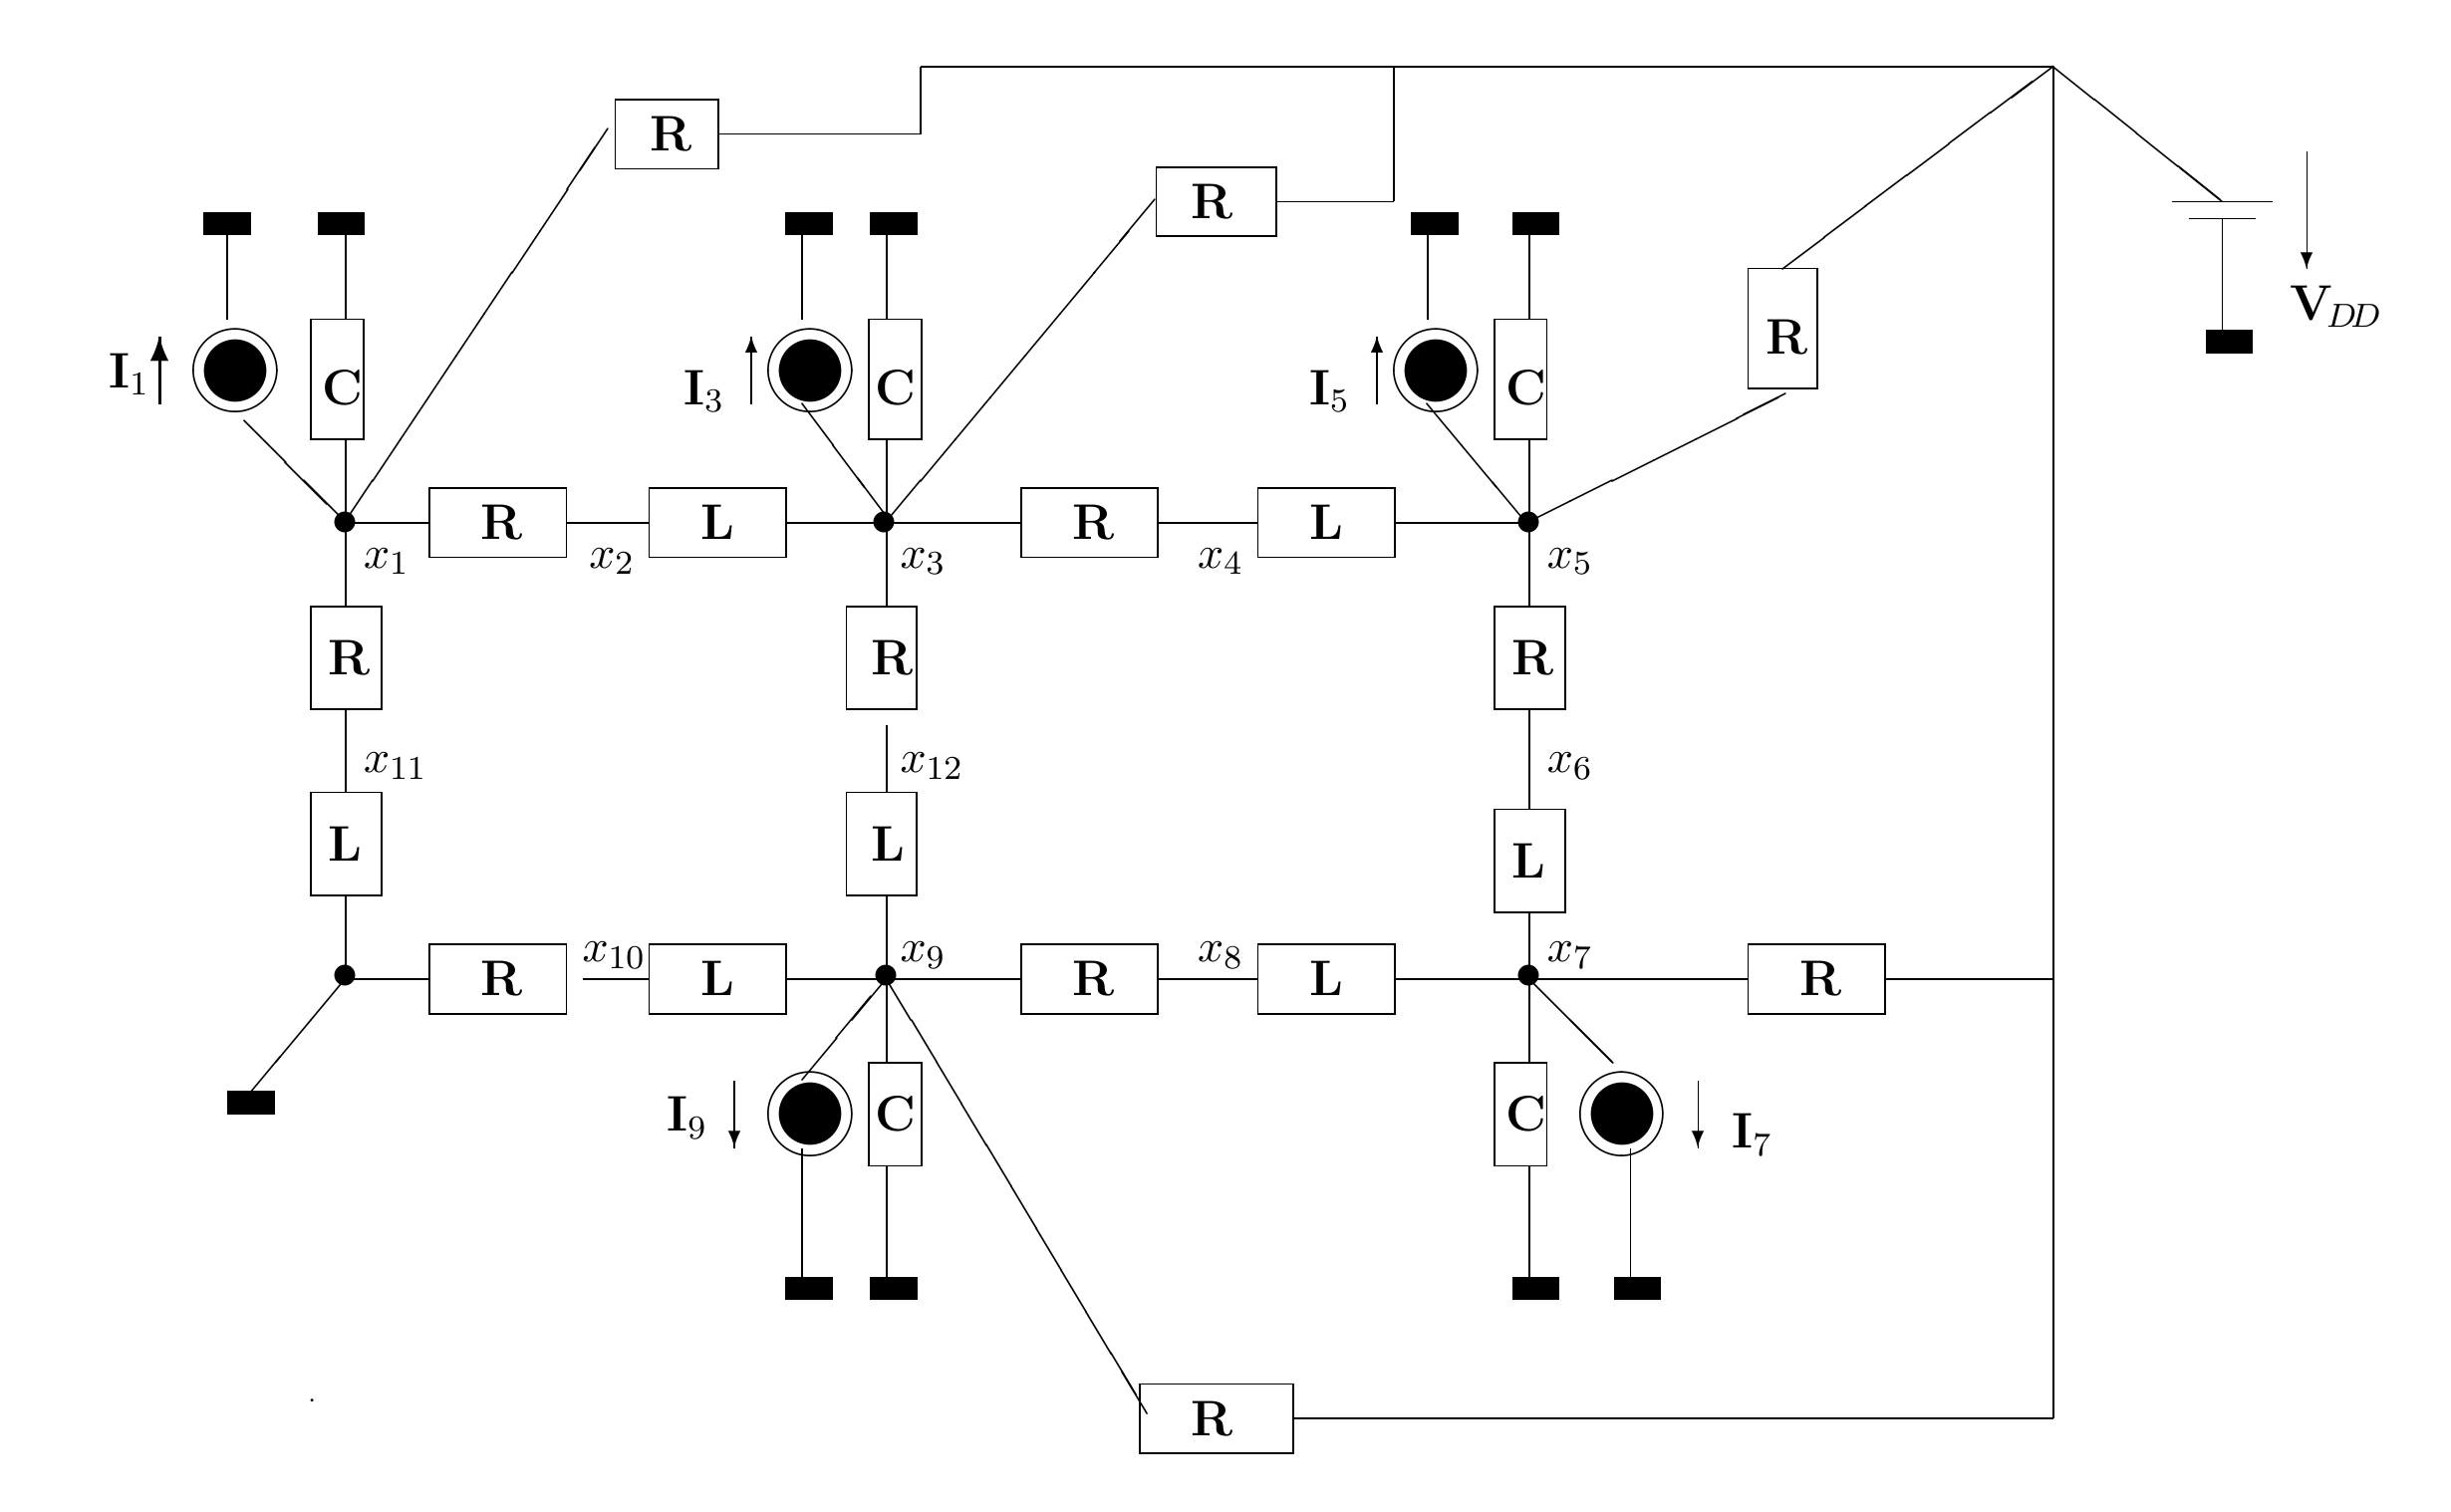
\includegraphics[scale=0.3]{./figs/pwr_grid}
\caption{Initial power grid module circuit with 2 layers ("micro-circuits"), \cite{task}}\label{fig:orig_circ}
\end{figure} 

\begin{figure}[!ht]
\centering
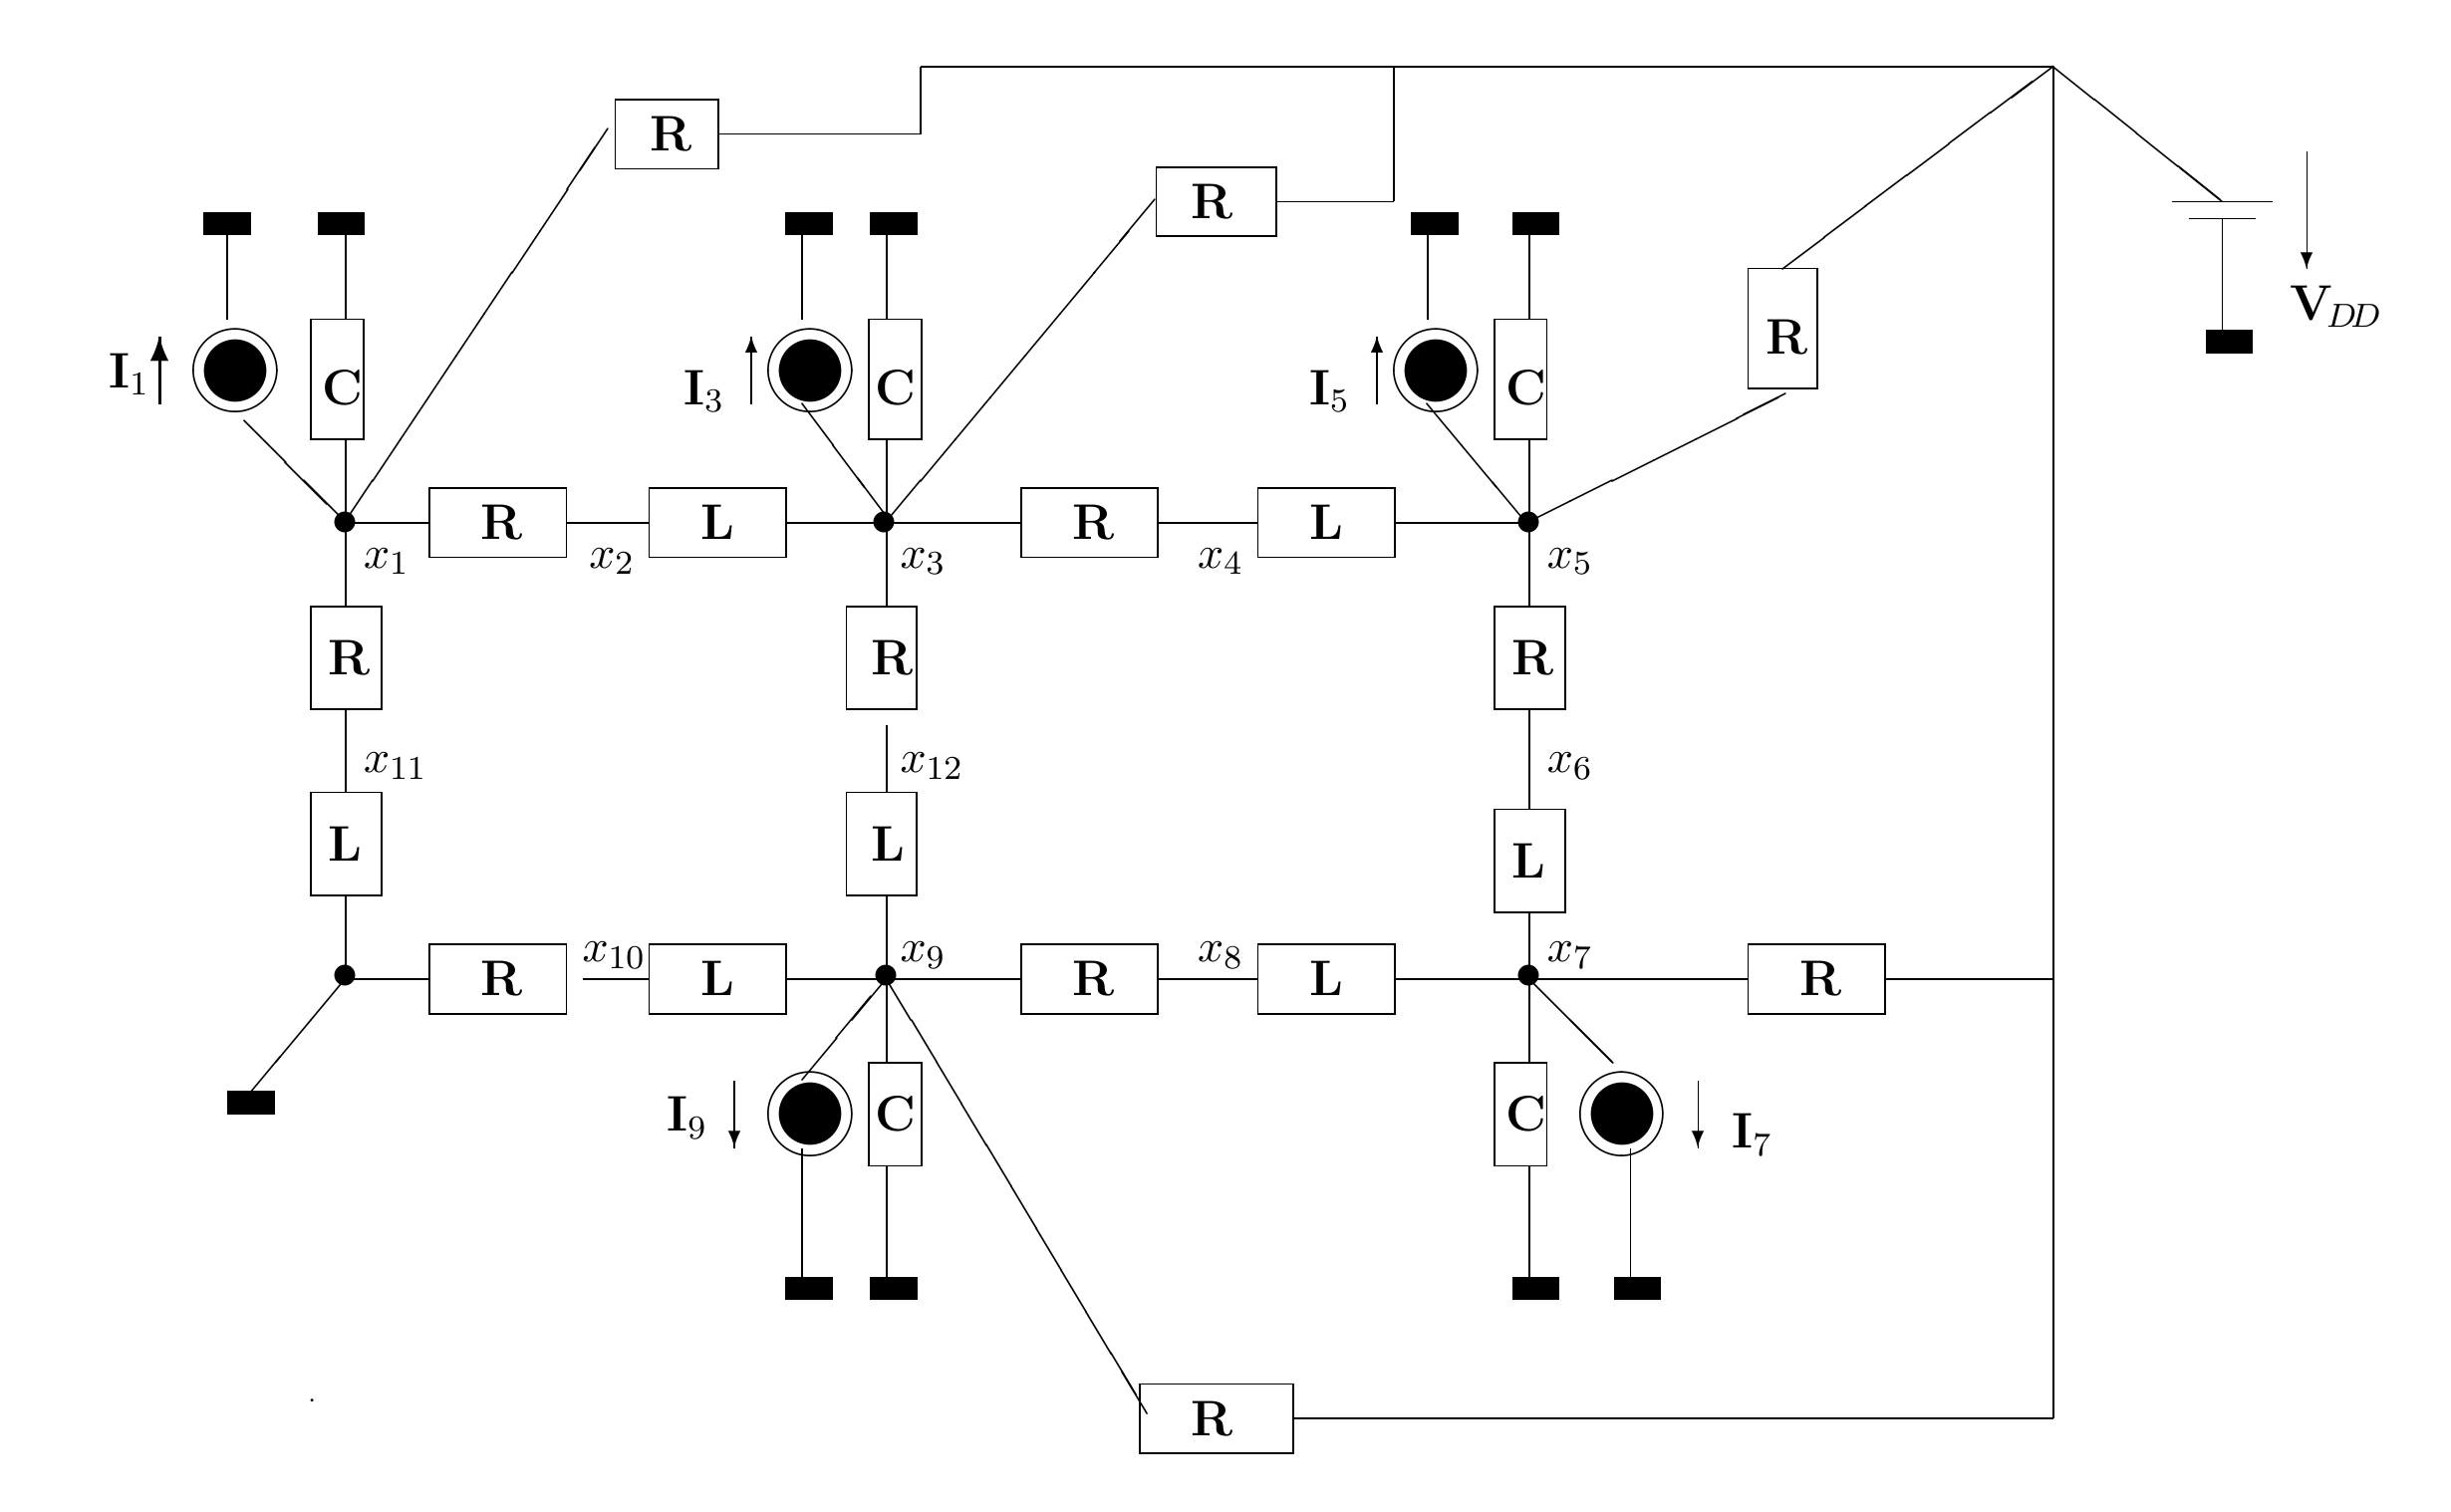
\includegraphics[scale=0.35]{./figs/pwr_grid} % change this to expanded circ.
\caption{Power grid model circuit to study (3 layers)}\label{fig:circ}
\end{figure}

We started by firstly determining the state space representation of the circuit's underlying dynamic system. In doing so, Kirchhoff's laws were applied and hence we obtained  the following system's equations (\ref{eq:sys}).

\begin{eqnarray}\label{eq:sys}
\left\lbrace\begin{array}{c | c}
C\dot{x_1} = -\frac{x_1}{R_1} - x_2 + x_{15} + \frac{u}{R_1} - I_1 & L\dot{x_2} = x_1 - R_2x_2 -x_3\\
C\dot{x_3} = -\frac{x_3}{R_3} + x_2 -x_4 - x_{16} + \frac{u}{R_3} - I_3 & L\dot{x_4} = x_3 - R_4x_4 -x_5\\
C\dot{x_5} = -\frac{x_5}{R_5} + x_4 - x_6 - x_{17} + \frac{u}{R_5} - I_5 & L\dot{x_6} = x_5 - R_6x_6 -x_7\\
C\dot{x_7} = -\frac{x_7}{R_7} +x_6 - x_8 + \frac{u}{R_7} - I_7 & L\dot{x_8} = x_7 - R_8x_8 -x_9\\
C\dot{x_9} = -\frac{x_9}{R_9} + x_8 -x_{10}+ \frac{u}{R_9} - I_9 & L\dot{x_{10}} = x_9 - R_{10}x_{10} -x_{11}\\
C\dot{x_{11}} = \frac{x_{11}}{R_{11}} + x_{10} - x_{12} + x_{17} + \frac{u}{R_{11}} - I_{11} & L\dot{x_{12}} = x_{11} - R_{12}x_{12} -x_{13}\\
C\dot{x_{13}} = -\frac{x_{13}}{R_{13}} + x_{12} - x_{14} + x_{16} + \frac{u}{R_{13}} - I_{13} & L\dot{x_{14}} = x_{13} - R_{14}x_{14}\\
& L\dot{x_{15}} = -x_1 - R_{15}x_{15} \\
&L\dot{x_{16}} = x_3 - R_{16}x_{16} -x_{13}\\
&L\dot{x_{17}} = x_5 - R_{17}x_{17} -x_{11}\\
\end{array}\right.
\end{eqnarray}

\begin{thebibliography}{3}
\bibitem {aa} A. Antoulas, Lecture Notes Model Order Reduction Course, Fall 2014, Jacobs University Bremen.7
\bibitem {task} A. Antoulas, Project task formulation , Model Order Reduction Course, Fall 2014, Jacobs University Bremen.
\end{thebibliography}
\end{document}